\documentclass{beamer}

\usepackage[spanish]{babel}
\usepackage[utf8]{inputenc}
\usepackage{lscape}
\usepackage{amsmath}
\usepackage{amsfonts}
\usepackage{amssymb}
\usepackage{graphicx}
\usepackage{multirow}
\usepackage{framed}
\usepackage{float}
\usepackage{times}
\usepackage{color}
\usepackage{algpseudocode}
\usepackage{wrapfig}
\usepackage{subfig}%%Para incluir subgraficos
\usepackage{fancyhdr}%%Para incluir encabezado
\usepackage{parskip}
\setlength{\parindent}{0pt}
\usepackage[section]{placeins}
\hypersetup{
  colorlinks=true,
  linkcolor=black,          % color of internal links (change box color with linkbordercolor)
  citecolor=black,        % color of links to bibliography
  filecolor=black,      % color of file links
  urlcolor=black           % color of external links
}


\title[ProgComp] % (optional, only for long titles)
      {Programación de Computadores}
      %\subtitle{}
      \author%[Author, Anders] % (optional, for multiple authors)
             {Sergio ~Monsalve\inst{1}} % \and S.~Anders\inst{2}}
             \institute%[Universities Here and There] % (optional)
                       {
                         \inst{1}%
                         Ingeniería de Sistemas\\
                         Departamento de Informatica\\
                         Universidad EAFIT
                         %% \and
                         %% \inst{2}%
                         %% Institute of Theoretical Philosophy\\
                         %% University There
                       }
                       \date[\today] % (optional)
                            {Semana 1}
                            \subject{Computer Science}
                            
\begin{document}
                            
\frame{\titlepage}


\begin{frame}
  \frametitle{Contenido}
  Computadores y lenguajes de programación
  IDEs: Idle, PyCharm, Sublime, Ideone

  \begin{figure}[p]
    \centering
    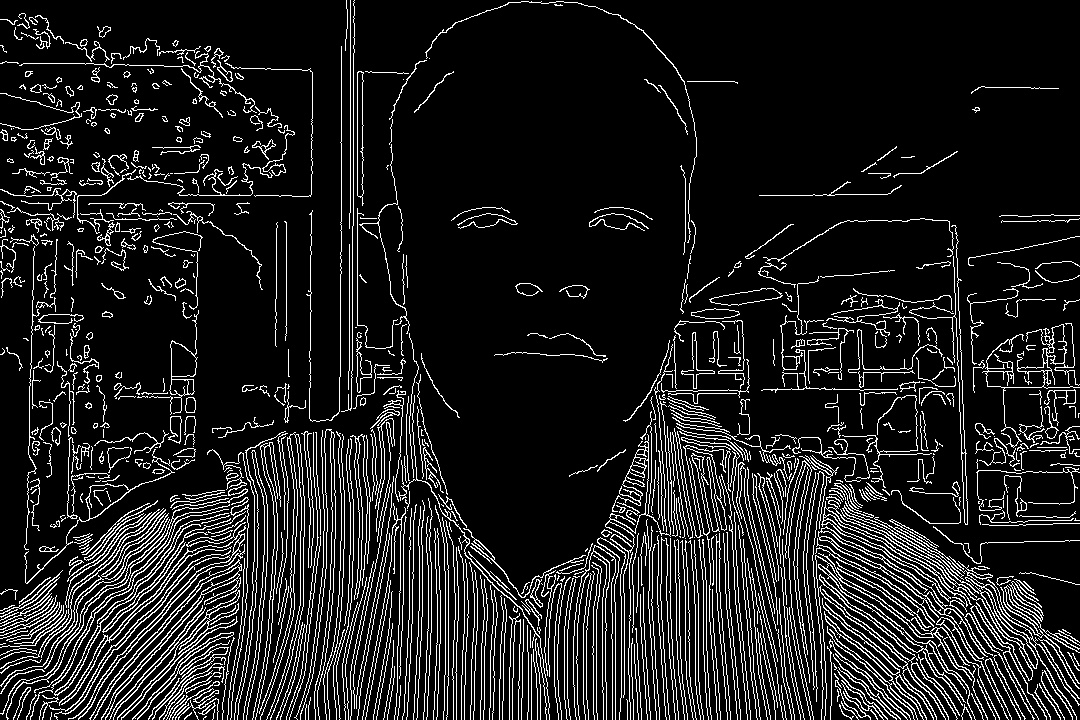
\includegraphics[width=0.7\textwidth]{SamCanny.jpg}
%    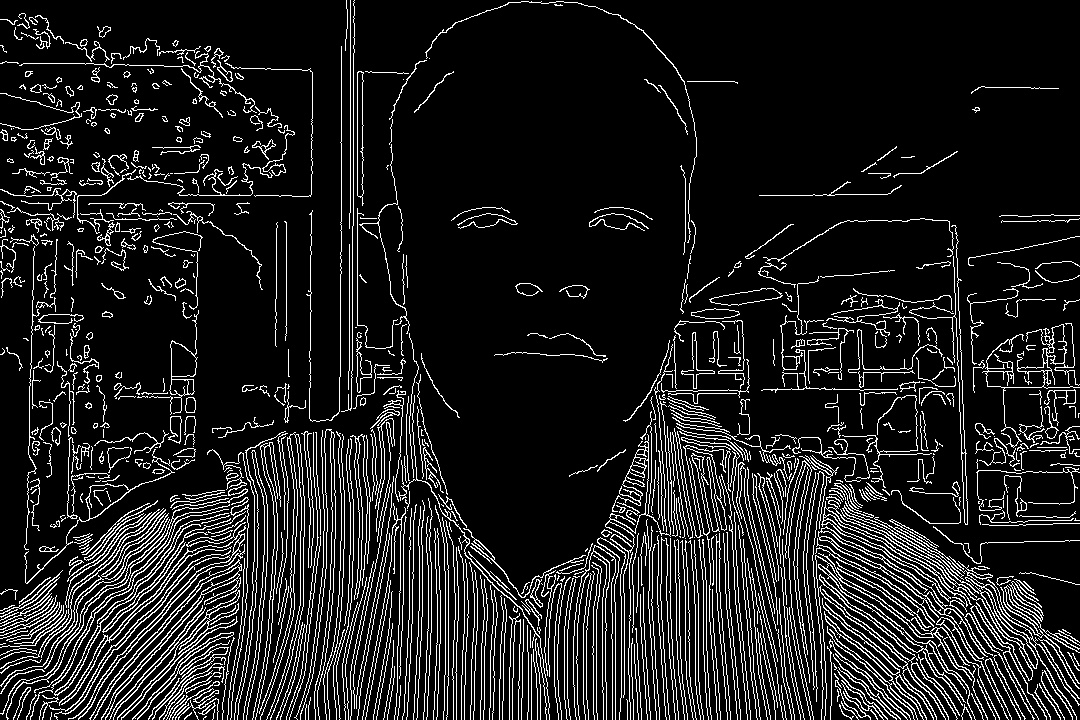
\includegraphics[scale=0.5]{SamCanny.jpg}
  \caption{mira!}
  \end{figure}
  
\end{frame}

\begin{frame}
  \frametitle{Presentación}
  \begin{itemize}
  \item Estudiantes
  \item Profesor
  \item El curso
  \item Objetivos
  \item evualuación
  \item Forma de Trabajo
  \end{itemize}
\end{frame}

\begin{frame}
  \frametitle{Historia}
  \framesubtitle{Hardware y Software}
    Lenguajes Compilados vs Interpretados
\end{frame}

\begin{frame}
  \frametitle{IDE}
  \framesubtitle{Entorno de Desarrollo Integrado(Integrated Development Environment)}
    Pycharm: Video de Instalación:
\end{frame}


\begin{frame}
  \frametitle{Nuestro Primer Programa}
  Salida Básica

  ``Hola Mundo''
\end{frame}

\begin{frame}
  \frametitle{Nuestro Primer Programa}
  Entrada Básica
  Nombre = ``Sergio''
  print ``Hola, ''+ Nombre
\end{frame}

\begin{frame}
  \frametitle{Conclusiones}
    Tipos y variables
    Expresiones
    Secuencias
\end{frame}


\begin{frame}
  \frametitle{Para la Próxima Clase}

  \begin{alertblock}{This is an Alert block}
    This is an important alert
  \end{alertblock}

\end{frame}


\begin{frame}{Example of columns 1}
  \begin{columns}[c] % the ``c'' option specifies center vertical alignment
    \column{.5\textwidth} % column designated by a command
    Contents of the first column
    \column{.5\textwidth}
    Contents split \\ into two lines
  \end{columns}
\end{frame}

\begin{frame}{Example of columns 2}
  \begin{columns}[T] % contents are top vertically aligned
    \begin{column}[T]{5cm} % each column can also be its own environment
      Contents of first column \\ split into two lines
    \end{column}
    \begin{column}[T]{5cm} % alternative top-align that's better for graphics
      % \includegraphics[height=3cm]{graphic.png}
      
    \end{column}
  \end{columns}
  \end{frame}

\begin{frame}

  \begin{block}{This is a Block}
    This is important information
  \end{block}

  \begin{exampleblock}{This is an Example block}
    This is an example
  \end{exampleblock}

  \end{frame}

\end{document}
